% Template for a Computer Science Tripos Part II project dissertation
\documentclass[12pt,a4paper,oneside,openright]{report}

\usepackage{amsmath, amsthm, amssymb}
\usepackage{array}
\usepackage{color}
\usepackage{docmute}   % only needed to allow inclusion of proposal.tex
\usepackage[margin=15mm]{geometry}  % adjusts page layout
\usepackage{graphicx}  % allows inclusion of PDF, PNG and JPG images
\usepackage[pdfborder={0 0 0}]{hyperref}    % turns references into hyperlinks
\usepackage{pdfpages}
\usepackage{verbatim}
\usepackage[bottom]{footmisc}

\newcolumntype{C}{>{{}}c<{{}}}

\setlength{\parindent}{0ex}

\clubpenalty1000%
\raggedbottom                           % try to avoid widows and orphans
\renewcommand{\baselinestretch}{1.1}    % adjust line spacing to make readable
\sloppy
\widowpenalty1000%

\begin{document}
\bibliographystyle{plain}

%%%%%%%%%%%%%%%%%%%%%%%%%%%%%%%%%%%%%%%%%%%%%%%%%%%%%%%%%%%%%%%%%%%%%%%%
% Title

{\let\cleardoublepage}

\rightline{\LARGE \textbf{Marius Latinis}}

\vspace*{60mm}
\begin{center}
\Huge
\textbf{Bus Arrival Time Prediction} \\[5mm]
Computer Science Tripos -- Part II \\[5mm]
Christ's College \\[5mm]
\today  % today's date
\end{center}
\newpage

%%%%%%%%%%%%%%%%%%%%%%%%%%%%%%%%%%%%%%%%%%%%%%%%%%%%%%%%%%%%%%%%%%%%%%%%%%%%%%
% Proforma, table of contents and list of figures

\pagestyle{empty}

\chapter*{Proforma}

{\large
\begin{tabular}{ll}
\textcolor{blue}{Name}: & \bf Marius Latinis                        \\
\textcolor{blue}{College}:            & \bf Christ's College                     \\
\textcolor{blue}{Project Title}:      & \bf Bus Arrival Time Prediction \\
\textcolor{blue}{Examination}:        & \bf Computer Science Tripos -- Part II, July 2017  \\
\textcolor{blue}{Word Count}:         & \bf \textcolor{red}{TODO(ml693): figure out} \\
\textcolor{blue}{Project Originator}: & \bf Dr Richard Mortier \\
\textcolor{blue}{Supervisor}:         & \bf Dr Richard Mortier \\ 
\end{tabular}
}
\stepcounter{footnote}


\section*{Original Aims of the Project}

\begin{itemize}
\item Implement the prediction algorithm. The GPS points showing how the bus has moved
so far are given as an input. The output of the prediction algorithm is the predicted
time when this bus will arrive at the future stop.

\item Evaluate the prediction algorithm and present the results.

\end{itemize}

\section*{Work Completed}

The following milestones have been achieved:

\begin{itemize}
\item The prediction algorithm is implemented.
\item The algorithm is evaluated and the results are presented in the evaluation section.
\item (Optional) the real-time prediction system is running.
\end{itemize}

\section*{Special Difficulties}

None
 
\section*{Declaration}

I, Marius Latinis of Christ's College, being a candidate for Part II of the Computer
Science Tripos, hereby declare that this dissertation and the work described 
in it are my own work, unaided except as may be specified below,
and that the dissertation does not contain material that has already been used to any substantial extent for a comparable purpose.

\bigskip
\leftline{Signed [signature]}

\medskip
\leftline{Date \today}

\tableofcontents

%%%%%%%%%%%%%%%%%%%%%%%%%%%%%%%%%%%%%%%%%%%%%%%%%%%%%%%%%%%%%%%%%%%%%%%
% now for the chapters

\pagestyle{plain}


\chapter{Introduction}

\section{Motivation}

In the European countries, public buses are a popular form of transportation. People
want to arrive in time to a particular place. They use the public transport for that.
For example, a bus is used travel to the airport, arrive at the first lesson in
school. Citizens rely on a vehicle travelling a certain distance in a certain
amount of time. The problem arises when the bus fails to arrive in time due to the
traffic congestion. This failure makes passengers miss various things. For instance, it
is very disappointing to miss a departing train due to the late bus. Therefore,
people are looking for a \underline{source of information} reliably telling when a
vehicle will reach a certain place. \\

\section{Timetable}

The \textcolor{green}{timetable} is one potential source of information: \\

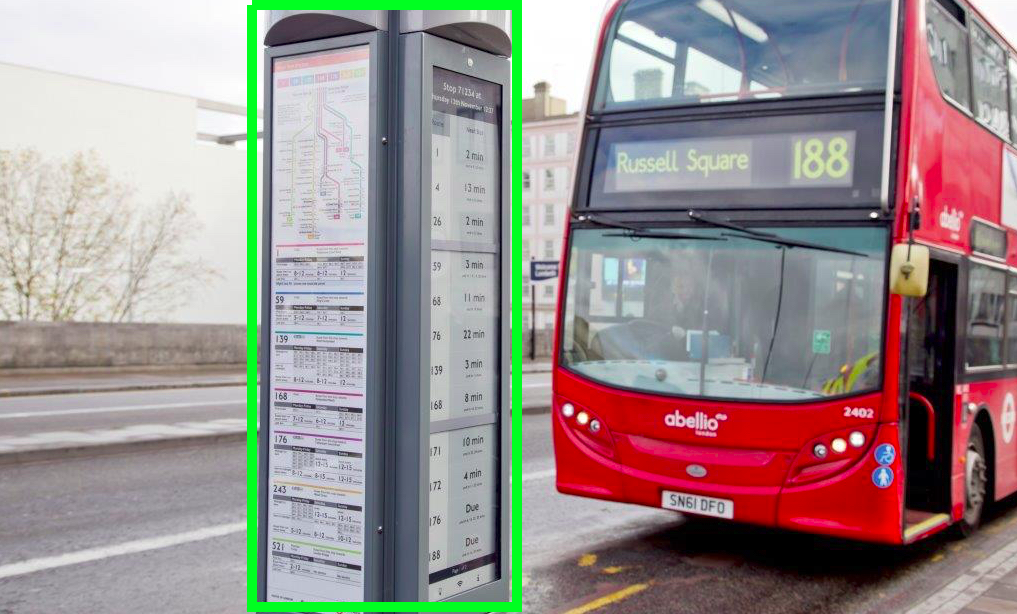
\includegraphics[width=\textwidth]{figs/timetable_uk.png}

Often the timetable appears as a stand at the bus stop $S_i$. It shows multiple
things, such as the bus arrival time at the same stop $S_i$, or a bus arrival time
at the next stops $S_{i+1}, S_{i+2}, ...$ The way to present a timetable varies.
For example, the information present on a stand is likely displayed on some website. \\

Unfortunately, every timetable is fundamentally limited. The arrival times it presents
are \textbf{static}. If the timetable claims the bus arrives at the stop at
time $T$, the value $T$ will not change. Such static arrival time prediction fails to
reflect the dynamic transport aspect. \\

\section{GPS}

The current technology allows making use of the GPS data. Modern buses are equipped
with the devices sensing their GPS position. The device sends the position at regular
intervals to a determined server that can store and instantly analyse the data. In
particular, the prediction analysis can be done to guess when the bus will arrive at
the next stop. The goal of my project is to perform such prediction analysis.
I aim to build an algorithm which predicts the bus arrival times based
on the most recent GPS data.

\section{Problem Overview}

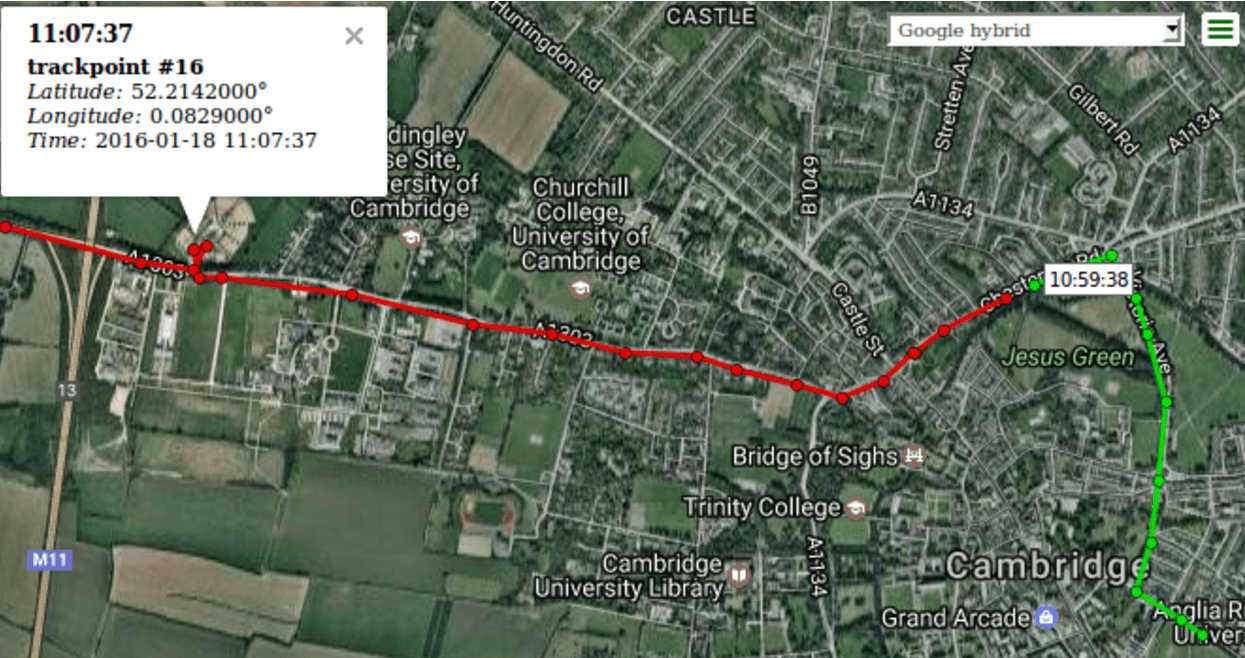
\includegraphics[width=\textwidth]{figs/problem_overview.png} \\

The most recent GPS points (indicated in green in the diagram above) show
where the bus has travelled up to now. The future data (indicated in red)
is not known during the prediction phase. My goal is to predict the future
data given the present data. \\

Here I want to predict when the bus will reach the Madingley Park starting from the
Chesterton Road. One can see it takes about 8 min. (10:59--11:07) to travel such distance.

\chapter{Preparation}

I see 3 main things that require thought before the implementation can commence:

\begin{enumerate}
\item What prediction algorithm I will code
\item What existing data and tools I will use
\item How will I evaluate the algorithm
\end{enumerate}

Sections 2.1, 2.2, 2.3 explain each thing one by one.

\section{Algorithm Choice}

\subsection{Existing Prediction Systems}

The traffic varies a lot based on the vehicle type, the city size, the road
infrastructure present in the city and other factors. There is no one universally
accepted algorithm predicting well for each of the different cases. For example, predicting
the train arrival time is easy. Other vehicles do not block the train on the rail. The train
speed is constant for most of the trip. Hence, the arrival time can be predicted dividing the
remaining travel distance by its current speed. This approach works well for trains. However,
I handle the buses travelling both in a single city and between multiple cities. The above
approach is hopeless for the buses traffic because the current bus speed will quickly
change due to the upcoming turns, traffic lights or other cars in front. Hence, just the
momentary speed alone is of little use. \\

Thus, it is important not to code any algorithm. I need to choose the one which suits
the GPS data I have and the type of traffic I am dealing with. I did a thorough preparation
to choose the correct approach. \\

Firstly, I read a paper describing how other scientists are solving this problem:

\begin{itemize}

\item Bin Yu, William H.K. Lam, Mei Lam Tam: Bus arrival time prediction at
bus stop with multiple routes 

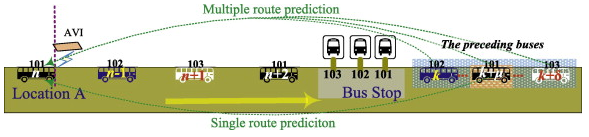
\includegraphics[width=\textwidth]{figs/paper.png}

\textcolor{blue}{\url{http://www.sciencedirect.com/science/article/pii/S0968090X11000155}}

\end{itemize}

On a high level, the paper uses the most recent buses arrival times at the bus stop $B$
from some location $A$. It feeds the times $t^{n}_{A->B}$ (how long the n-th
preceding bus travelled from $A$ to $B$) into the machine learning model (neural network,
support vector machine and others are tried) and hopes that the model will predict a
sensible arrival time for the current bus to reach $B$ from $A$. \\

My implementation incorporates one idea from that paper:
\textit{"[...] the running time(s) of the preceding bus(es) that has(ve) \textbf{just}
reached the stop can be used to reflect the traffic conditions."} \\


\subsection{My Choice}

After talking with Prof Kelly, I decided not to use Machine Learning and found an alternative.
The problem many Machine Learning models have is that they act like a black-box. For example,
the weights on the edges of a neural network eventually converge to certain values. It is often
difficult to understand the intuitive meaning of a particular value:

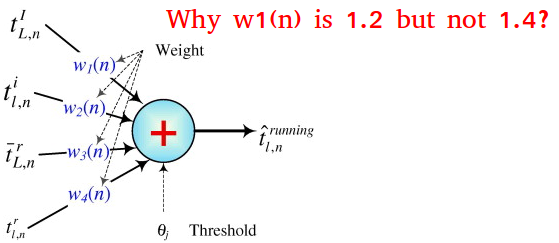
\includegraphics[width=\textwidth]{figs/ann.png} \\

It is thus hard to explicitly re-program the model in case it does not work with the data.
Since the traffic data generated by humans driving vehicles on the street can be very
unpredictable (e.g. the Phantom Traffic
Jam\footnote{\textcolor{blue}{\url{https://www.youtube.com/watch?v=goVjVVaLe10}}}),
I see no guarantee that a particular model will succeed on the first attempt. \\

The model presented in this dissertation is much simpler to understand. I initially extract
certain values (e.g. the time it takes for a bus to reach the stop $B$ from the location $A$)
from the historical data set, just as the previous paper does. However, I do not feed the values
into the ML model. I write the specific data-processing code. The result of this is that
I have my own learning model\footnote{The model is presented in the
implementation chapter.} and understand it very well. If I see that the model does not predict
well, I look at the data and figure out why that happens. I improve the model after inspecting
the data. \\

\section{Available Data and Tools}

\subsection{Starting Point}

\subsection*{Initial GPS Data}
A company named Vix is sending the real-time GPS data to the Cambridge servers. The GPS
data shows how certain East-England buses (Stagecoach and Whippet) are moving 
in the real-time. The Cambridge servers convert the binary GPS data into a human readable
JSON format. The JSON data is saved. At the beginning of the academic year I was given the
JSON data spanning 3 months (June, July and August 2016).
That was the starting point data. \\

To start with, I wrote the prediction algorithm entirely from scratch and tested it on the historical
starting point data.

\subsection*{GPS Data for the Real-time System}
In the second term, I started building the real-time system as an optional extension.
The optional part requires the real-time GPS data. To start with, Dr. Lewis gave me
the access to the machine receiving the new GPS data from the Vix company every 30sec. \\

The code receiving the real-time GPS data and immediatelly converting it to the JSON format was already written. I started this part by writing the new code processing the real-time JSON data.

\subsection{Map Data}

One can represent the road as an edge and the intersection of two roads as a vertex.
Alternatively, Google Maps uses vertices to model roads and edges to model intersections
joining two roads. They claim this unintuitive representation helps to reason that
it takes a different amount of time to turn left, right or drive straight at the intersection: \\

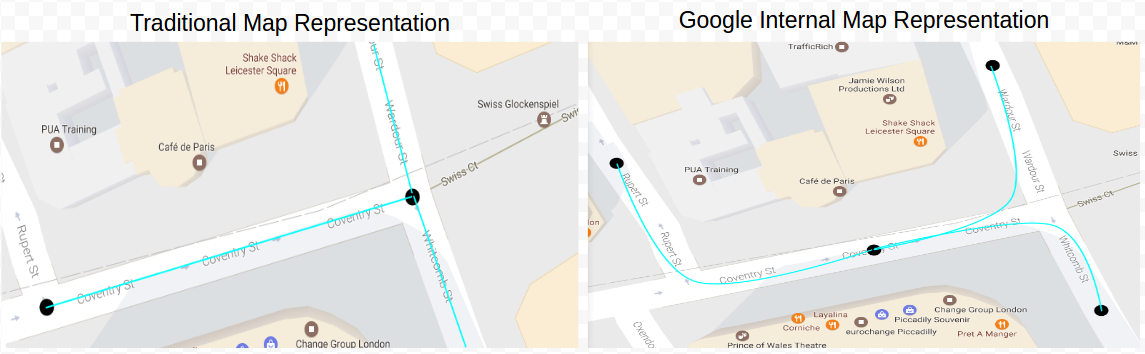
\includegraphics[width=\textwidth]{figs/google.png}

In any case, a graph is used to represent the map. A bus trip corresponds to a walk
along the graph edges. I initially considered predicting the arrival time by summing the
time it takes for a bus to travel along every street on its route (i.e. along every edge on
a path in a graph). This approach would have required
me getting the map data. Collecting the data (street names, lengths, traffic directions, etc.)
and building a graph representation of it is a big task. However, my overseers pointed out
that it is \textbf{not necessary} to have this data at all: \\

\textit{"My thought was more radical: ultimately what you need is to build a predictive
 model of when the bus will arrive based on previous samples of its position and other
 vehicles position. That model doesn't necessarily have to be based on the connectivity
 graph of the roads; it might be enough to (for example) pick out the mean speed of
 vehicles within any 200m square, and learn how bus arrival time (on any particular route)
 depends on all those speeds across the whole area. That wouldn't involve *extracting* map
 data at all."} \\

Following the given advice I decided not to collect the map data. This deviation from the
original plan saved a lot of my time.

\subsection{Language Choice}

A language must be convenient for the type of code I have to write. This project requires writing
the following pieces of code:

\begin{enumerate}
\item Code inspecting the JSON format and converting it into another form.
\item Core algorithms (e.g. Dynamic Time Warping) predicting the arrival time.
\item Prediction \textbf{system design} code.
\end{enumerate}

I think Java is (up to a certain extent) a language convenient to write all of the above:

\begin{enumerate}
\item It has built-in $String$ handling methods and IO facilities to read the data from a file.
\item It has advanced data structures (e.g. $HashMap$) to code an algorithm.
\item Java supports multithreading. Multiple components (new GPS data processor, arrival time
      predictor, statistics generator) can run at the same time and interact with each other.
\end{enumerate}

\newpage 

\section{Evaluation Overview}

I read a second paper:

\begin{itemize}

\item Pengfei Zhou, Yuanqing Zheng, Mo Li: How Long to Wait? Predicting Bus Arrival Time
      with Mobile Phone based Participatory Sensing Pengfei Zhou, Yuanqing Zheng, Mo Li

\textcolor{blue}{\url{http://www.ntu.edu.sg/home/limo/papers/sys012fp.pdf}}

\end{itemize}

I extracted the common evaluation metrics used in both papers. The Mean Absolute Error value
($MAE$) is the only sensible common evaluation metric. Most of my evaluation is grounded on the
$MAE$ value. \\

However, the second paper illustrates one important aspect:

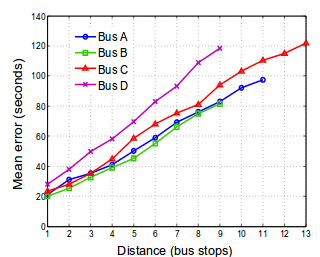
\includegraphics[scale=0.8]{figs/second_paper.png}

The prediction errors are meaningful only if one knows how far in advance they were
generated. Suppose the prediction error is 80 sec. If it takes approximately one hour to reach
the last bus stop, then the 80 sec. prediction error to the last stop is a very small number.
If I predict the arrival time the next stop less than 2 minutes away from the current location,
then 80 sec. is a large error. \\

My evaluation chapter takes this aspect into account.




\chapter{Implementation}

\section{Data Preprocessing}

Below is the starting point input data example: \\
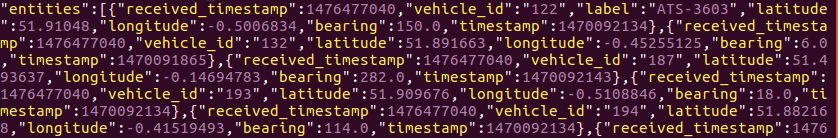
\includegraphics[scale=0.6]{figs/starting_data.png}

One file contains a single snapshot of all buses, 
with one entry per bus. An entry such as:

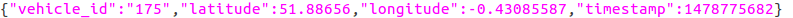
\includegraphics[width=\textwidth]{figs/entry.png}

means that a vehicle nr. $509$ was at the geographical position
$(51.88656, -0.43085587)$ on the $10$st November $2016$, GMT time
$11$:$01$:$22$ (the time is calculated from the timestamp field 1478775682). \\

A new snapshot file arrives once in $30$s. The data preprocessing part
takes multiple input files\footnote{For example, to build historical trips, I take $3600 \cdot 24 / 30 = 2880$ files
received in \textbf{one} day and preprocess them.} and converts them into another format:

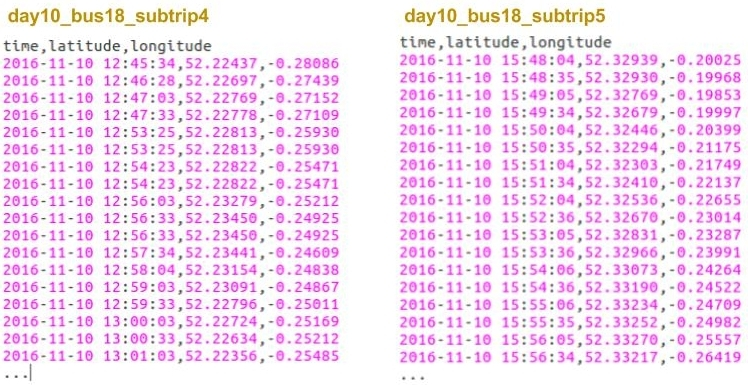
\includegraphics[width=\textwidth]{figs/converted_format.jpg}

At the end I have a file for each trip made by one bus in one
day\footnote{Note that a bus on a particurlar day could have made
multiple trips.}. \\

Visually the data preprocessing part converts the following set of GPS points

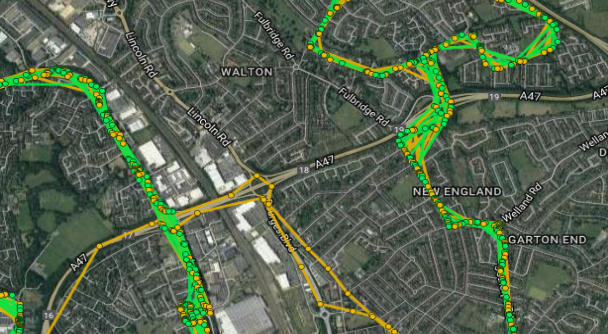
\includegraphics[width=\textwidth]{figs/unprocessed.png} \\

into a separated list of trips, 2 of which are shown below:

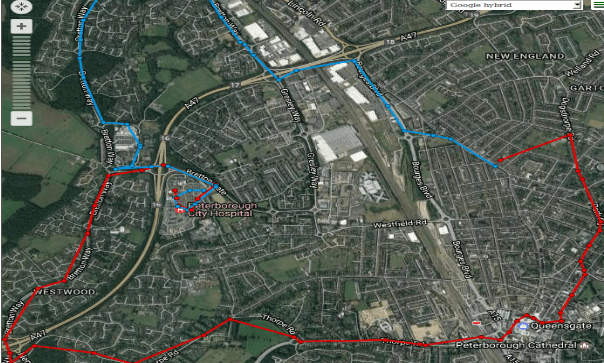
\includegraphics[width=\textwidth]{figs/processed.png} \\

An optional use\footnote{The main use is that the preprocessing part is one of the
components of the whole arrival time prediction system.} of the preprocessing part
is the help it provides to visually inspect the data. I am able to look at each trip
separately (or to merge multiple trips of my choice) and understand why the buses are
moving in such a way.

\section{Route Detection Algorithm}

\subsection{Why an Algorithm is Needed}

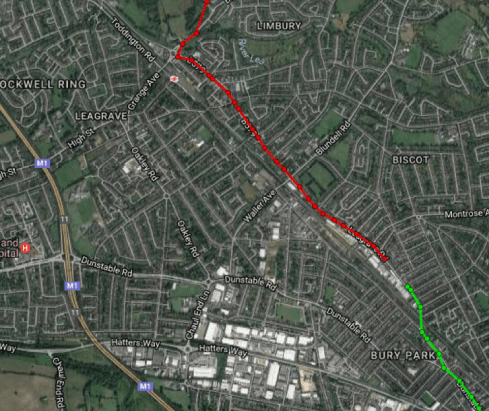
\includegraphics[scale=0.8]{figs/route_detector.png} \\

The GPS points indicated in green show how the bus has moved so far.
The red points show where the bus will travel in the future,
a path I do not know yet. Predicting when the bus will arrive at the stop
requires knowing \textbf{where} a bus will travel next. How? \\

\textbf{Approach Using Static Data} \\

A standard way to find out where the bus will travel next is to know its 
route in advance. Some GPS entries contain additional fields,
such as the \textbf{label} field: \\

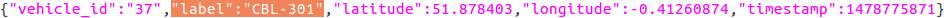
\includegraphics[width=\textwidth, scale=1.2]{figs/labelled_entry.png} \\

An extra field \textbf{label} names the route a bus follows. Auxiliary
data might indicate what route the label \textbf{CBL-301} corresponds to.
One can then look at the route and determine a sequence of stops 
a bus will visit next. \\

Unfortunately, this approach has drawbacks:

\begin{itemize}
\item Not all entries contain auxiliary fields. After all, the GPS device on the
actual vehicle is responsible only for providing the latitude and longitude
coordinates, not the route a bus follows.

\item Good static data to infer routes based on additional fields is not 
straightforward to find. Field values might not match
(For example, a route named \textbf{SW-4} in the real-time data is actually
\textbf{SWX-4}).
Buses are often changing routes\footnote{A bus is unlikely to follow the same route
every day} and data does not always indicate that.

\item The static data only shows the sequence of bus stops, not a detailed
sequence of streets a bus will follow. It is much better to know an actual
path for the accurate arrival time prediction.
\end{itemize}

\textbf{New Approach Overview} \\

To overcome the static data limitations, I propose a new way to infer the
route a bus follows. I will align a sub-trip how the bus has moved
so far with a historical path for which the route is known. The path aligning
best to the current sub-trip will be used to predict where a bus travels next.
To perform the alignment, I constructed an algorithm\footnote{From now on referred
to as a boolean predicate.} that can tell whether one sequence of GPS points 
follows another.

\subsection{$FollowsPath$ Predicate Definition}

I define a predicate $FollowsPath(sub$-$trip, path)$ to be true iff a $sub$-$trip$
follows a $path$:

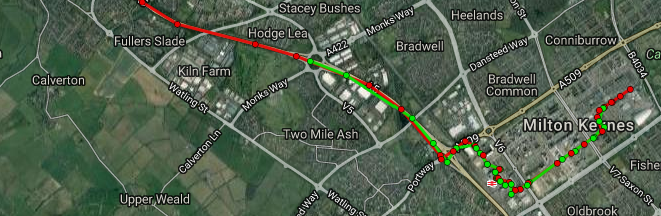
\includegraphics[width=\textwidth]{figs/follows.png}

For the picture above, the $FollowsPath(\textcolor{green}{subtrip}, \textcolor{red}{path})$ 
predicate returns true, because it is intuitively clear that the \textcolor{green}{subtrip}
follows a \textcolor{red}{path}. \\

In the next example, the $FollowsPath(\textcolor{green}{subtrip}, \textcolor{red}{path})$
predicate returns false, as the two GPS sequences do not intersect at all:

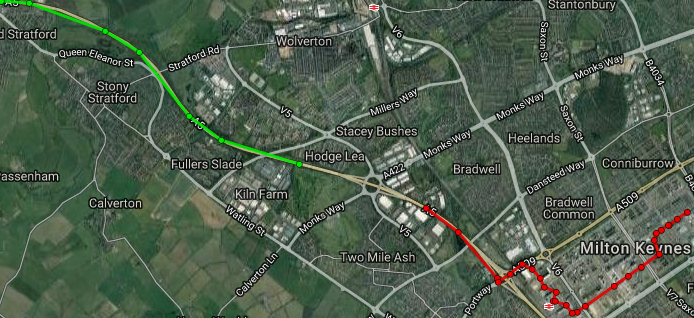
\includegraphics[width=\textwidth]{figs/not_follows_path.png}

\:

\subsection{$FollowsPath$ Predicate Implementation}

Firstly, consider the case when a \textcolor{red}{sub- trip's} GPS points
$(\textcolor{red}{P_0}, \textcolor{red}{P_1}, ..., \textcolor{red}{P_{n-1}})$
\textbf{exactly} follow another \textcolor{blue}{path}: \\

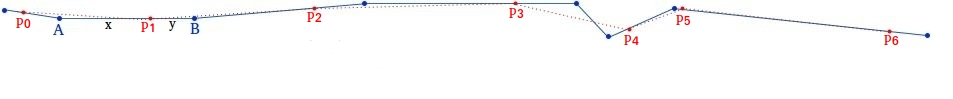
\includegraphics[width=\textwidth]{figs/follows_exactly.jpg}

Each point $P_i$ is on some segment of another trip's path.
For example, $P_1$ is on the segment $AB$.
Let $x = |AP_1|$ and $y = |P_1B|$. Then the
error\footnote{error function takes a point and a segment as an input} function
defined as \\

\begin{centering}
$err(P_1, AB) = \frac{x + y}{|AB|} - 1$ \\
\end{centering}

\:
\:
\:

equals $0$. For each point $P_i$, I find a segment $S_{P_i}$ such that
$err(P_i, S_{P_i})$ is minimised. The $FollowsPath$ predicate returns true
iff

\begin{centering}
    $S = \sum_{i=0}^{n-1} err(P_i, S_{P_i}) < n\epsilon$ \\
\end{centering}

\:
\:
\:

for a suitably chosen threshold value $\epsilon$ ($\epsilon = 0.1$ is one choice). \\

Note that $S = 0$ when a \textcolor{red}{sub-trip} follows a
\textcolor{blue}{path} exactly. Therefore, in this case, the $FollowsPath$
predicate returns true, which is what I want. \\

The case when a \textcolor{red}{sub-trip} does follow a
\textcolor{blue}{path}, but not exactly (the real world situation), 
is illustrated in the following picture: \\

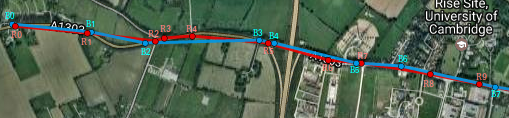
\includegraphics[width=\textwidth]{figs/follows_roughly.png}

In this example I am aligning a \textcolor{red}{sub-trip}
$(\textcolor{red}{R_0}, ..., \textcolor{red}{R_9})$ with a \textcolor{blue}{path}
$(\textcolor{cyan}{B_0}, ..., \textcolor{cyan}{B_7}, ...)$.
The computation of $S$ proceeds as follows:
\[
\setlength\arraycolsep{0pt}
\begin{array}{ *{7}{cC} c }
 S &=& err(\textcolor{red}{R_0}, \textcolor{cyan}{{B_0}{B_1}}) &+& 
       err(\textcolor{red}{R_1}, \textcolor{cyan}{{B_0}{B_1}}) &+& 
       err(\textcolor{red}{R_2}, \textcolor{cyan}{{B_2}{B_3}}) &+& 
       err(\textcolor{red}{R_3}, \textcolor{cyan}{{B_2}{B_3}}) &+& 
       err(\textcolor{red}{R_4}, \textcolor{cyan}{{B_2}{B_3}}) &+  \\
   & & err(\textcolor{red}{R_5}, \textcolor{cyan}{{B_3}{B_4}}) &+& 
       err(\textcolor{red}{R_6}, \textcolor{cyan}{{B_4}{B_5}}) &+& 
       err(\textcolor{red}{R_7}, \textcolor{cyan}{{B_5}{B_6}}) &+& 
       err(\textcolor{red}{R_8}, \textcolor{cyan}{{B_6}{B_7}}) &+&
       err(\textcolor{red}{R_9}, \textcolor{cyan}{{B_6}{B_7}}) &   \\
   &=& (1.0294 - 1)  &+& (1.0300 - 1) &+& (1.0021 - 1)  &+& (1.0730 - 1)  &+& 
       (1.0208 - 1)   &+  \\ 
   & & (1.0714 - 1)  &+& (1.0286 - 1)  &+& (1.0158 - 1)  &+&  (1.0126 - 1)  &+& 
       (1.0125 - 1)   &<& 10 \cdot 0.1 =& n\epsilon
\end{array}
\]

and the predicate again returns true, as desired. \\

\newpage

The last case is when a \textcolor{red}{sub-trip} does not follow a
\textcolor{blue}{path}:

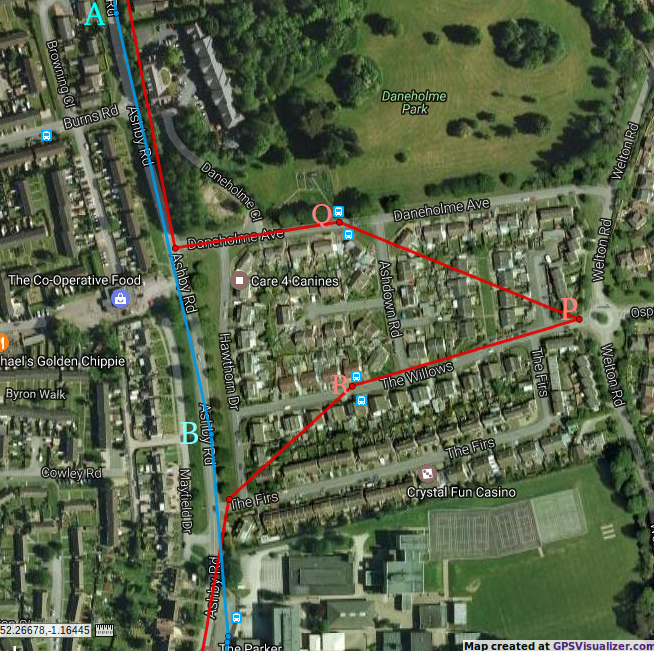
\includegraphics[scale=0.6]{figs/not_follows.png} \\

In this case the triangle inequality ensures large $err(P_i, S_{P_i})$ values for
certain points $P_i$. For example, for the point \textcolor{red}{$P$} in the diagram,
the smallest error value is \\

\begin{centering}
$err(\textcolor{red}{P}, \textcolor{blue}{AB})$ = $(12.9 + 9) / 10\footnote{The distances $12.9$, $9$ and $10$ are scaled here. Scaling does not change the ratio value.}
- 1 = 1.1$ \\


\end{centering}

\:
\:
\:

This error is more than $10$ times larger than the typical values being less than
$0.1$. Furthermore, large errors will be generated for each sub-trip's point that
deviated from the path, such as for the points \textcolor{red}{Q} and
\textcolor{red}{R} in the diagram. Hence, the total errors sum $S$ will exceed
$n\epsilon$ and the predicate will return false. \\

The practical evidence that the $FollowsPath$ predicate works is given in the
evaluation section.

\newpage

\section{Arrival Time Prediction}

\subsection{Basic Idea}

The $FollowsPath$ predicate allows to detect the route a bus follows.
The route tells the next stops a bus will visit. This section shows how to
predict the arrival time to each future bus stop. \\

Historical trips (which follow the same route) are used to make a prediction:

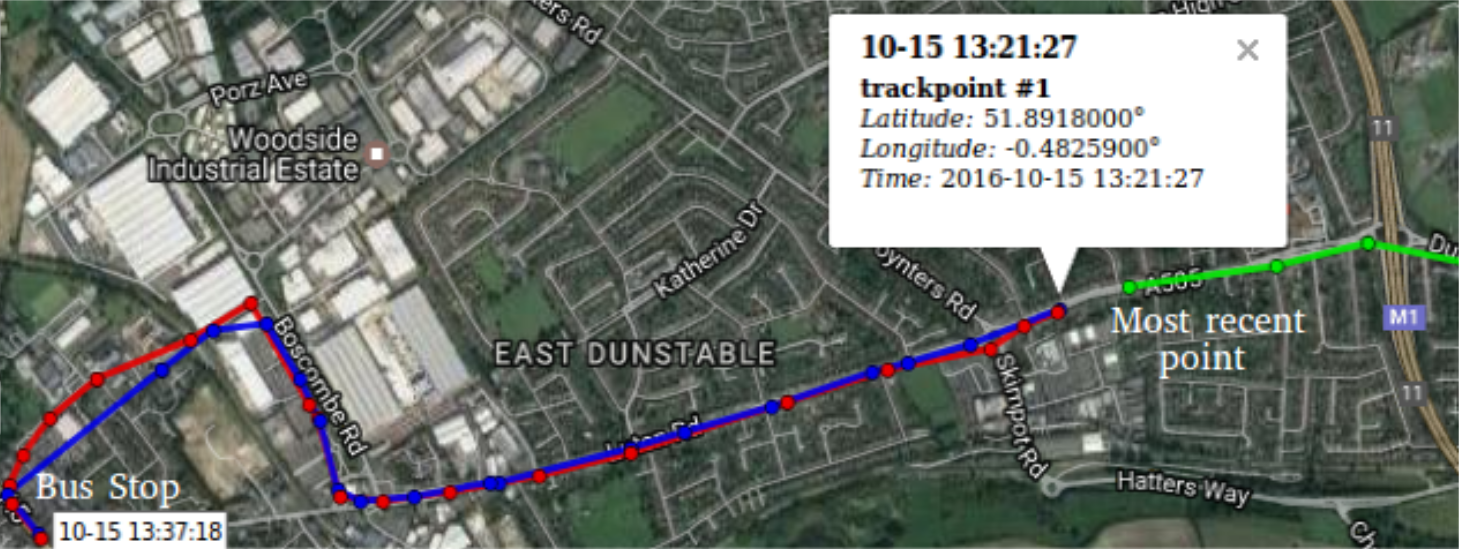
\includegraphics[width=\textwidth]{figs/future_stop.png} \\

In the picture above 2 example historical sub-trips (\textcolor{blue}{blue}
and \textcolor{red}{red}) are shown.
Both of them start where at the current vehicle's location (indicated
using the most recent green point). Both of them represent the history how past
vehicles travelled until the bus stop. I compute the duration how long it
took for each historical trip to reach the bus stop. Knowing multiple duration values
I return the median as the predicted arrival time. \\

For example, it took 13:37:18 $-$ 13:21:27 = 15m 51s for the
\textcolor{blue}{blue trip} to reach the bus stop. I also calculate these
duration values for the \textcolor{red}{red} and other trips present in the
historical trips set. The computation gives me a list of numbers.
I sort the list:

\:
\:

(8m 30s, 14m 46s, 14m 58s, 15m 06s, \textbf{15m 36s}, 15m 51s, 16m 07s, 16m 31s,
 17m 34s)

\:
\:

and return the median value. Thus, I predict that the bus indicated in green will
reach the bus stop after 15m 36s. \\

The reason for choosing a median value rather than some other average number
(such as the arithmetic mean) is to get rid of the outliers. The shortest arrival time
8m 30s is a much smaller number than others. I discard this number when computing
the median. Different computation might have been negatively influenced by the outlier. \\

The median value predicted better compared to the arithmetic mean during the testing
phase. Thus, I decided to stick with the median value.

\subsection{Optimisation Nr. 1}

If in the historical trips set certain trips have \textbf{just} travelled along
the same route (e.g. in the last $30$min.), I predict the median time just from
those recent trips. Otherwise, the basic approach is used.

\subsection{Optimisation Nr. 2}

Suppose the most recent data

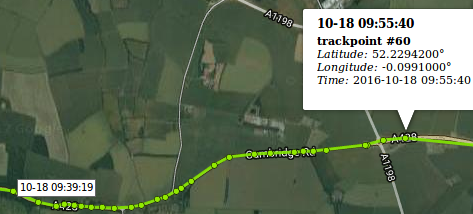
\includegraphics[scale = 0.7]{figs/recent_trip.png} \\

shows the distance a bus has travelled in the last $16$ minutes. Certain historical
trips

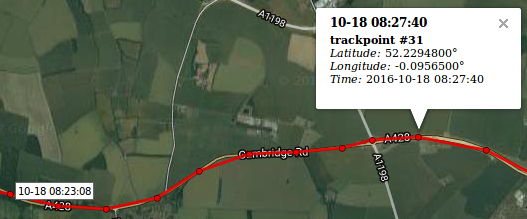
\includegraphics[scale = 0.7]{figs/inaccurate_historical.png} \\

have travelled the same distance in a very different amount of 
time\footnote{This could have happened due to the different traffic congestion level
in a different time of the day.} (e.g. $4$ min.). Predicting the arrival time using
these historical trips can be misleading. This optimisation discards misleading
trips. \\

I pick the last $N$ points (e.g. $N = 30$) of the trip I want to predict the arrival
time. The 1st point out of $N$ shows where the bus was $M$ minutes ago (if $N=30$, then
most likely $M=15$, because the new GPS point is usually generated once in 30s).
For each historical trip I find the point $P$ where the historical bus was $M$ minutes
ago from the moment of time when it reached the current bus location. If $P$ is roughly
the same location as the current bus location $M$ minutes ago, I include the historical
trip into the set $C$ of consideration. I discard this historical trip otherwise.
After the set $C$ is generated, I proceed only with it as before (3.3.1). \\

This optimisation is the simplest way I found to take into account the traffic
periodicity. One can expect that the traffic on Tuesday might be similar to the
traffic on Monday (a period of one day). Thus, one can hope that historical trips
of the last day are suitable to predict what will happen today. However,
this is not always true. The traffic on Monday (the working day) is very different
from the traffic on Sunday (the weekend). Setting a period to be 1 week also does not
fix the problem entirely. It can be that the Monday a week ago was a holiday day.
Traffic during holidays is also different from the traffic during the regular days. \\

Fortunatelly, my optimisation addresses both the fact that the traffic follows some
periodic pattern and also the fact that the period is not strict. One way to look at
the optimisation described above is as follows. The bus location $M$ minutes ago shows
its current \textbf{"speed" along the route} (not the actual mph velocity, but how
quickly it passed the route segment). The speed is correlated with the traffic
congestion. The reason why some historical trip (which happened either a day or a week
ago) had similar speed to the current bus is because the traffic was similarly
congested to how it is congested now. And if the trip was similarly congested because
of the periodic pattern, then this optimisation detects all periodic trips, regardless
what the actual period is. \\

Optimisations are tested in the evaluation section.


\newpage

\section{Real-time System (Optional)}

I am processing the GPS data at real time. The goal of this chapter is to present
the current system's state so that whoever comes after
me\footnote{Such as another student next year.} can understand the system and
improve it. \\

One machine every 30s. accepts a new JSON file containing the GPS data. For each new
file the machine does the following:

\begin{enumerate}

\item[(a)] Reads the new GPS data from the file and updates the arrival time
prediction values.

Below is a flow chart handling
\textbf{one} bus:

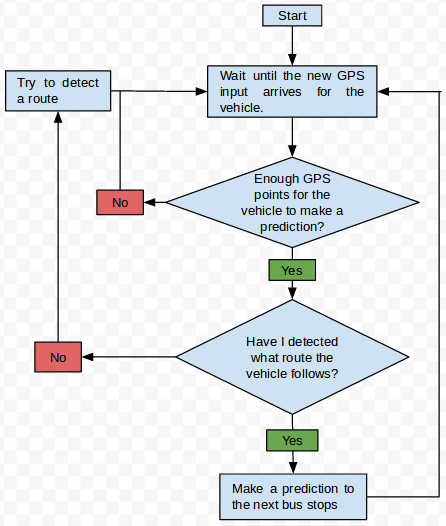
\includegraphics[scale = 0.6]{figs/flowchart.png} \\

This is how for \textbf{each} bus I \textbf{independently} process its new GPS data
and predict the arrival time to the next bus stops. Currently one machine is
waiting for $t$ sec., then using the new GPS data to handle $50$ buses in 
$30 - t$ sec.\footnote{Of course, I am trying to minimise $t$ and maximise the number of buses
handled $30 - t$ sec.}

\item[(b)] Saves the JSON file to a disc. Once in 24h reads the files saved on a disc
and generates the new historical data to improve the future predictions.

The current state of a system is such that for each new day I save the JSON files
to a separate directory. When a day $d+1$ comes, I read all JSON files corresponding
to day $d$ and perform the data preprocessing part (3.1) on those files. This generates
about $20000$ new trips every day. For each of the trip generated I then detect
which route it followed and save this trip into the historical trips directory
corresponding to that route. Hence, after each day I generate new historical trips
following a route. New historical trips improve the arrival time prediction
performance (part 3.3).

\end{enumerate}

\chapter{Evaluation}

\section{Evaluation Data Preparation}


I take the historical November data and generate the set $S$ consisting of 532428\footnote{
The size of this set is large but sensible. If 1000 buses are present in each JSON file,
the duration of 1 full trip is $\sim1h$, and November has 30 days, 
then $30 \cdot 24 \cdot 1000 = 720000$ is comparable to $532428$.} trips. I also have $3050$ routes
($2640$ of them are read from old files, $410$ of them are new routes present
in the new Traveline National Dataset (TNDS)). \\

I then run a long computation (it took 36 hours to complete on Dr Lewis machine): \\

For each trip $t \in S$ I search for a route that the trip \textbf{completely}
went through (i.e. visited all route stops in order). If I find a route, I save the trip. If no route is found, I discard the
trip. At the end I save only the routes for which more than 100 trips 
were found. \\

I am very selective during this computation. I consider that the trip stopped
at stop $s$ iff it contains a GPS point very close to $s$. \\



The computation returns 25 routes each having more than 100 trips passing through it completely. The next
sections evaluate my algorithm on these 25 routes. \\

It is surprising that \textbf{none} of the routes are from the new TNDS set. I contacted the officer
working with this data and got the following reply:

\textit{"In practice, within the TNDS, you will find that Route data is either limited or
non-existent."} \\

The process above voluntarily discards a lot of data. I want to explain this decision.
Improving any system is a natural ambition. I see two ways how the prediction algorithm can
perform better:

\begin{itemize} 
\item The itself algorithm is improved.
\item The data becomes better.
\end{itemize}

I believe, that \textbf{if both} options are possible, one should \textbf{first} try the latter.
This case applies to my project. I want to evaluate the algorithm on a data that meets
the quality standards. Thus, I discard the poor data and use only the qualified data for the
evaluation. \\


\section{Route Detection Evaluation}

\subsection{Sensitivity Score}

This section checks whether the $FollowsPath$($sub$-$trip$, $path$) predicate returns $true$
when the $sub$-$trip$ indeed follows a $path$. For each path $p$ (corresponding to a route) I
have a set $T_p$ of trips that went through it. For each trip $t \in T_p$ I take a
sub-trip $s$ and check that the $FollowsPath(s, p)$ returns true. \\

For 11 routes (out of 25) the $FollowsPath$ predicate has $100\%$ success rate. \\

For other 14 routes, I present the sensitivity scores in the decreasing order:

(0.99, 0.99, 0.98, 0.98, 0.89, 0.86, 0.86, 0.84, 0.58, 0.48, 0.38, 0.13, 0.12) \\

The picture below ilustrates the reason for having lower than $100\%$ scores:

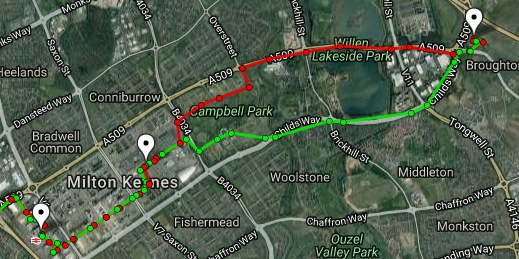
\includegraphics[width=\textwidth]{figs/same_route_wrong_path.png}

The \textcolor{green}{trip} reached the second bus stop using a different path
than the \textcolor{red}{one} I have as a path representing the route.
Some routes have few stops (e.g. 3) and the stops are far away from each other.
For these routes there are many different paths a bus can use to travel
between two consecutive stops. That is the reason why for some routes the
sensitivity score is low.

\subsection{Specificity Score}

This section checks that for trips not on a path the predicate returns false. \\

If a trip is very far away from the path (e.g. $10$ miles away), the
$FollowsPath(trip, path)$ will definitely return false. Thus, to perform
a meaningful evaluation, I select a \textcolor{blue}{path}
$1051719$-$20150531$-$20151224$ and a set of \textcolor{red}{trips}
$T$ following a very similar but nevertheless distinct path: \\

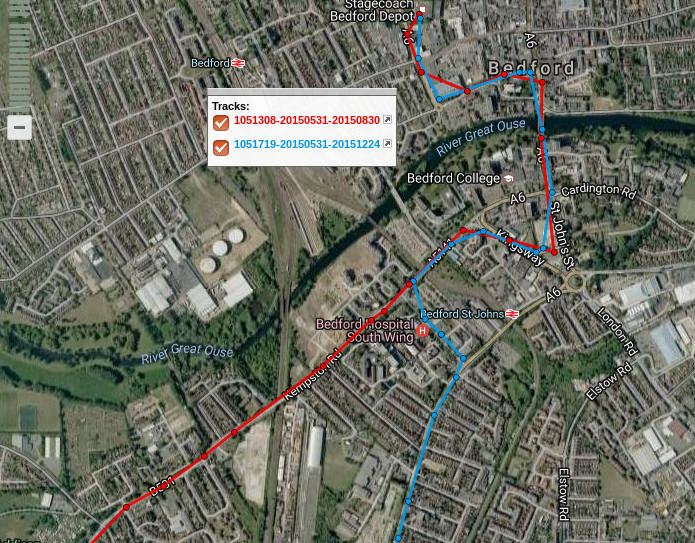
\includegraphics[scale = 0.6]{figs/similar_paths.png}

Both paths are the same at the beginning and separate later. For each
trip $\in T$ I pick a \textcolor{red}{$subtrip$} of the first 12
points\footnote{Each trip deviates from a path approximatelly after 12 GPS
points.} and check whether the
$FollowsPath(\textcolor{red}{subtrip}, \textcolor{blue}{path})$ 
returns false. Out of $107$ trips only once the predicate incorrectly returns
true. The misclassified \textcolor{red}{$subtrip$} has not deviated from a
\textcolor{blue}{path} yet for a predicate to detect that: \\

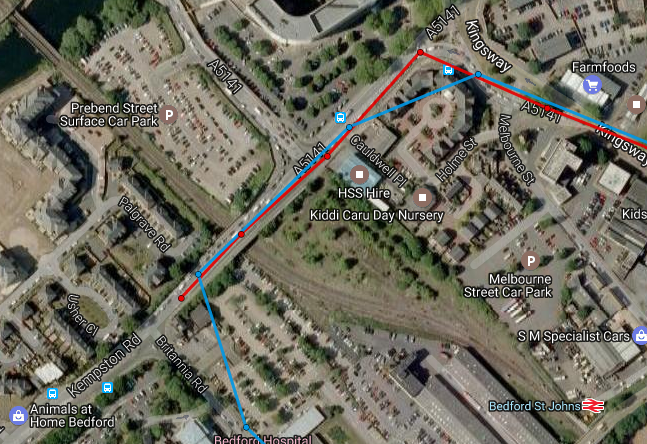
\includegraphics[scale = 0.6]{figs/misclassified_trip.png}

The sensitivity and specificity scores show that the $FollowsPath$
predicate works \textbf{if} used in the right place at the right time.

\newpage

\section{Arrival Time Prediction Evaluation}

\subsection{Evaluation Metrics Used}

This evaluation section is the most important. It shows how well the algorithm
predicts the arrival time. A few evaluation metrics are used repetitively
throughout the section. Hence, I want to present them. For the presentation I
will use the example route 1046531-20150531-20150830, which begins outside of
Cambridge and ends at the Cambridge Railway station: \\

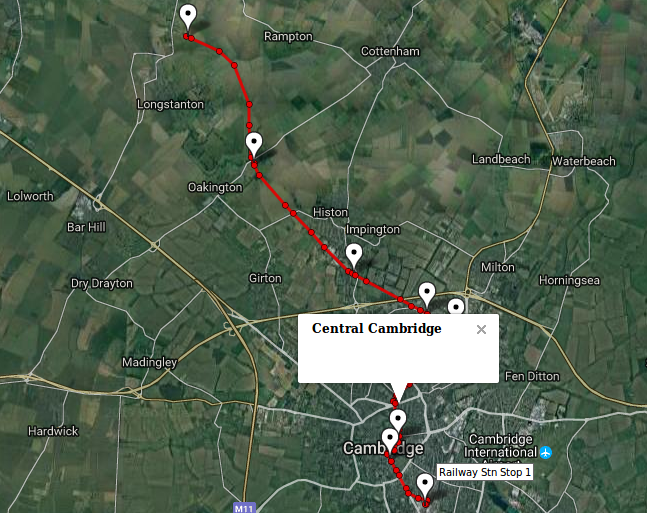
\includegraphics[width=\textwidth]{figs/cambridge_route.png} \\

\begin{enumerate}
\item[(i)]
    \textbf{The MAE value}. Suppose I have a set
    of trips $T$, such that each trip eventually reaches a bus stop of interest. 
    Suppose for trip $t \in T$ the algorithm predicts the bus arrival time
    at stop to be $t_{predicted}$, but the bus actually arrives at $t_{actual}$.
    The absolute prediction error for trip $t$ is
    $E_t = |t_{actual} - t_{predicted}|$. The \textbf{mean} absolute prediction
    error for the whole set $T$ is

    \begin{center}
        $MAE = \frac{\sum\nolimits_{t \in {T}}{E_t}}{|T|}$
    \end{center}

    For example, suppose I predict when the buses will reach the Railway Station
    starting from the Central Cambridge stop. I have $674$ trips
    following this route to test my prediction. For each test trip, I assume
    only its history up to the Central Cambridge stop is known. I predict
    the arrival time to the Railway Station. After the prediction is done,
    I read the rest of the history and check when the trip has actually
    arrived at the Railway Station. For this example trip, the resulting
    $MAE$ value is \textbf{98} sec. This number shows the average error the
    prediction algorithm makes. One can also use the MAE value to compare
    2 algorithms. I claim that the prediction algorithm $A$ performs better
    for some set than the algorithm $B$, if $MAE_A < MAE_B$.

\item[(ii)] \textbf{The scatter plot}. The $MAE$ value gives a first
   clue how well the algorithm performs. However, just the $MAE$ value
   alone is misleading. 98 seconds can be either a small or a large
   error. It depends how far in the future I am predicting. It takes about 10 
   minutes to reach the Railway Station from the Central Cambridge stop. Thus,
   98 seconds is an error \textbf{with respect to} the Central Cambridge stop. 
   The scatter plot formalises this relation:


\end{enumerate}

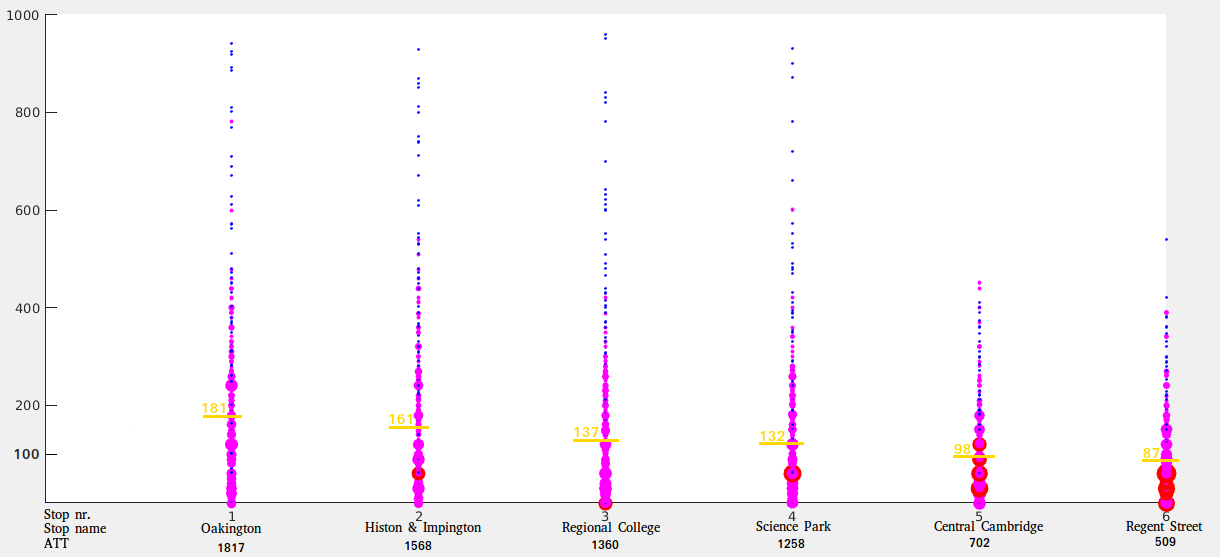
\includegraphics[width=\textwidth]{figs/scatter_plot.png} \\

\begin{itemize}

\item[]
   The x-axis labels the stop number $i$. For each $i$, I predict when the bus
   will reach the Railway Station (the last stop) starting from the $i$-th stop.
   The y-axis labels the absolute prediction error (measured in seconds).
   A point $(i, y)$ tells that for some trip the prediction from the $i$-th stop
   to the last stop has an abolute error equal $y$. The more repeated errors
   $(i, y)$ I have, the larger point I plot. For completeness,
   in the diagram I show the MAE value (labelled in yellow) and the 
   average travel time\footnote{For each trip I calculate the time it actually
   takes to reach the last stop, then return the mean value.} from the $i$-th stop
   to the last stop.

   A few things can be observed in this plot:
   
\begin{itemize} 
   
   \item 
   Firstly, the $MAE$ value is smaller
   for each larger index $i$. The less time it takes for a bus to reach the last
   stop, the more accurate the prediction becomes.

   \item
   In my case, many prediction errors are smaller than the $MAE$ value,
   except for a few large errors that make the $MAE$ value increase. The large errors
   occur due to unusual traffic patterns:

   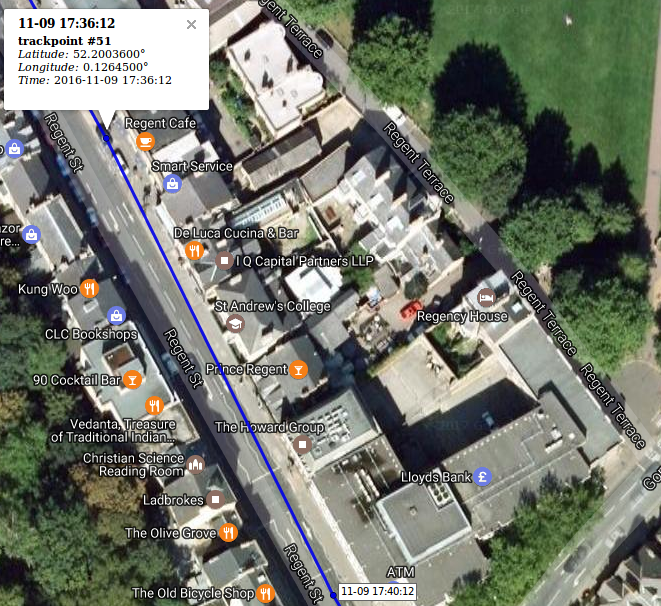
\includegraphics[scale=0.6]{figs/unusual_pattern.png} \\

    For some bus it took $4$ minutes to pass just a few buildings. Since most
    historical trips usually pass this segment in a much shorter
    time\footnote{e.g. 30s}, the predicted arrival time to the bus stop is
    much smaller than the actual arrival time. Therefore, the large error value 
    is generated.

    \item
    The scatter plot shows the absolute prediction errors only, not whether
    the bus arrived earlier or later than predicted. There is a simple reason for
    this: the prediction errors are symmetric, due to how my algorithm constructed
    is. On average, half of the errors are positive, half negative. Thus, it is
    enough to plot only the absolute errors and not lose any information.

\end{itemize}

All prediction points are shown on one plot. Hence, the scatter plot can be
used as a representative summary of what the algorithm predicts.


\end{itemize}

\begin{enumerate}

\item[(iii)] \textbf{The table of errors}. Traffic is different at a different time of
the day. I split the day into 4 disjoint time intervals:

\begin{enumerate}
\item[1.] $8$am--$10$am. The morning rush hour.
\item[2.] $10$am--$5$pm. The working hours.
\item[2.] $5$pm--$8$pm. The evening rush hour.
\item[3.] $8$pm--$8$am. I call all other hours as the 'night' time.



\end{enumerate}

I evaluate the prediction for each of the time intervals separately. The 
\textbf{table of errors} shows the aggregated results\footnote{As before,
I predict the arrival time to the \textbf{last} stop starting from each of the
other stops}:

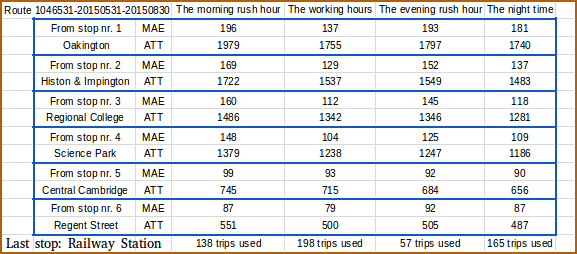
\includegraphics[width=\textwidth]{figs/table_of_times.png}

The table of errors shows the different prediction errors for different
times of the day. It is useful for those who are interested in a
particular route and want to check the extent up to which the prediction system 
can be trusted for that route. For example, suppose I want to take a morning train
to London. I can look at the morning column of this table and see that on average
it takes $745$s. to reach the train station from the Central Cambridge. I can
also see that an algorithm on average predicts the arrival time to the train station
with an error of $99$s.

Note that the average travel time, as well as the mean absolute
prediction error values, are larger for the first and third intervals of time.
Hence, for this route the traffic is more congested and less predictable
during the rush hours.

\end{enumerate}


\subsection{Evaluation on other Routes}

I used one route to present the metrics. The fact that an algorithm works on a single route
does not neccessary imply that it works on other routes. Hence, I evaluate the algorithm on
$25$ other routes for which I have enough data. The
detailed results are given in the appendix \ref{B1}. \\

\subsection*{The Best Route}

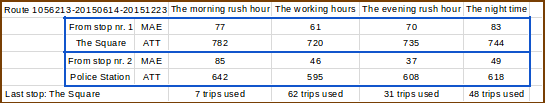
\includegraphics[width=\textwidth]{figs/table_of_1056213.png}

Out of the $10$ routes, the algorithm performs best on the route
$1056213$-$20150614$-$20152323$:

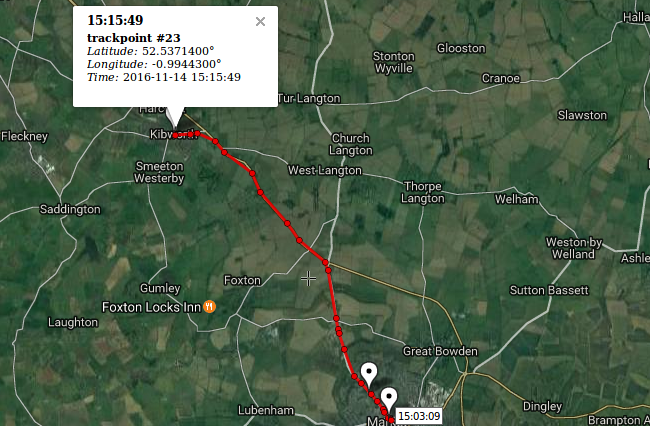
\includegraphics[scale=0.65]{figs/best_route.png}

For many time intervals, the algorithm predicts the arrival time with an average error
less than $10\%$. \\

I believe, a long highway path is the reason, why an algorithm successful for this route is.
Firstly, highways have a feature that they they are less connected with other
roads\footnote{Compare a highway with a street in a city. The latter usually has many
intersections with other streets. The former has only a few connected roads to go in and out
of the highway.}. Other roads have a relatively little affect on the highway traffic.
Hence, only historical trips of the buses travelling along this route are enough to generate
reasonable predictions\footnote{And the implementation of my algorithm uses only historical trips
following this route.}. Secondly, the bus speed on the highway does not vary
much. For example, if for the last 5 minutes the bus speed was $60$mph., it is 
likely it will keep travelling at roughly the same speed\footnote{Contrast this with the
case when a bus is on the street in a city. The bus speed will fluctuate a lot due to
traffic lights, other cars causing a congestion, pedestratians crossing the street.}.
This second feature of a highway allows making a good use of the
Optimisation nr. 2. The optimisation predicts the arrival time using only those
historical trips that have travelled a certain distance using the same amount of
time\footnote{$\implies$ the same travel speed.} as the current trip. Since the travel
speed on a highway does not vary much, these historical trips will give an accurate
information how quickly a bus might reach the bus stop. \\

Finally, I include the scatter plot. As before, many prediction errors are below the $MAE$ value:

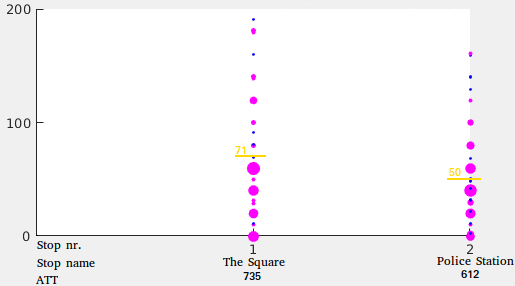
\includegraphics[scale=0.5]{figs/best_scatter_plot.png}

\subsection*{The Worst Route}

The algorithm performs poorly on the route $999024$-$20150526$-$20150830$: \\

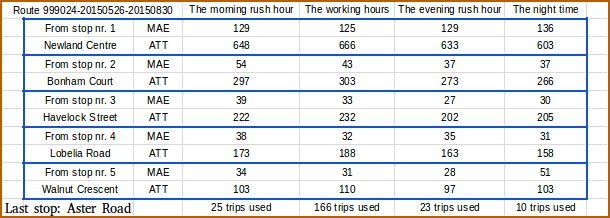
\includegraphics[width=\textwidth]{figs/table_of_999024.png} \\

The poor performance is due to the following reasons. Firstly, there are many bus stops a bus
frequently\footnote{Every $2$min. or so.} stops at. The amount of time a bus is standing at one
stop affects its arrival time to the future stop, but the algorithm does not explicitly deal with
the bus standing time. \\

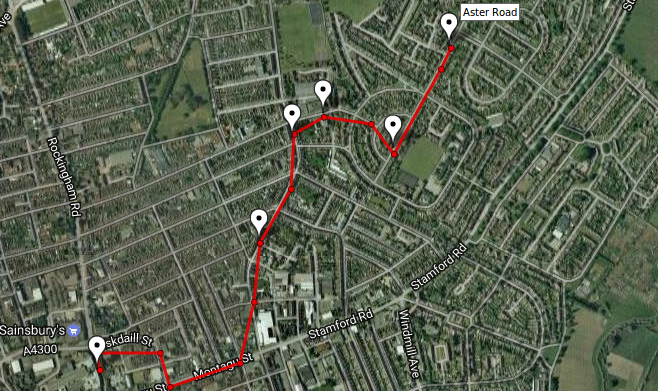
\includegraphics[scale=0.8]{figs/worst_route.png} \\

\newpage

Secondly, the route includes the crowded city places, such as the shopping centre: \\

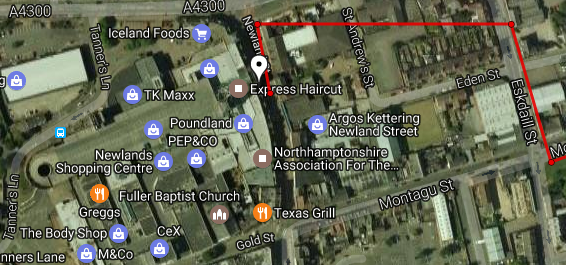
\includegraphics[scale=0.6]{figs/shopping_centre.png} \\

The scatter plot shows the difficulty predicting the arrival time in the crowded areas:

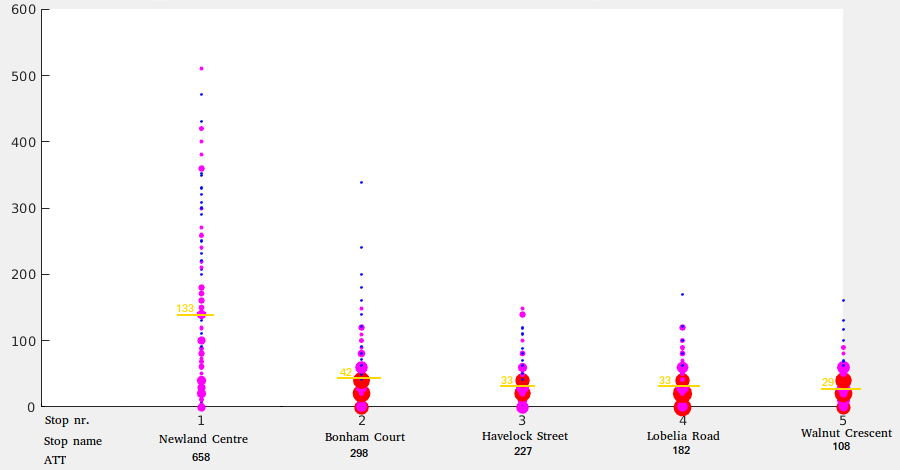
\includegraphics[width=\textwidth]{figs/worst_scatter_plot.png}

One can see a big difference between the prediction results from the first stop (where the
crowded place is) and from the other stops. The prediction errors predicting from
the first stop are not concentrated below the $MAE$ value. Instead, the errors are spread out
accross the whole range of $y$ values. After the bus leaves the crowded area, the prediction
errors become concentrated below the $MAE$ value, which is the usual characteristic of my
prediction algorithm. \\

I make the following conclusions:

\begin{itemize}

    \item My algorithm predicts the arrival time well for buses that are travelling from one city
    to another and are using highways for a long time.

    \item My algorithm may perform worse when predicting the arrival time in cities.


\end{itemize}



\newpage

\subsection{Different Systems Comparison}

\subsection*{Comparing Optimisations}

I first run the non-optimised algorithm to predict when the bus will reach the
Madingley Park starting from the Chesterton Road: \\

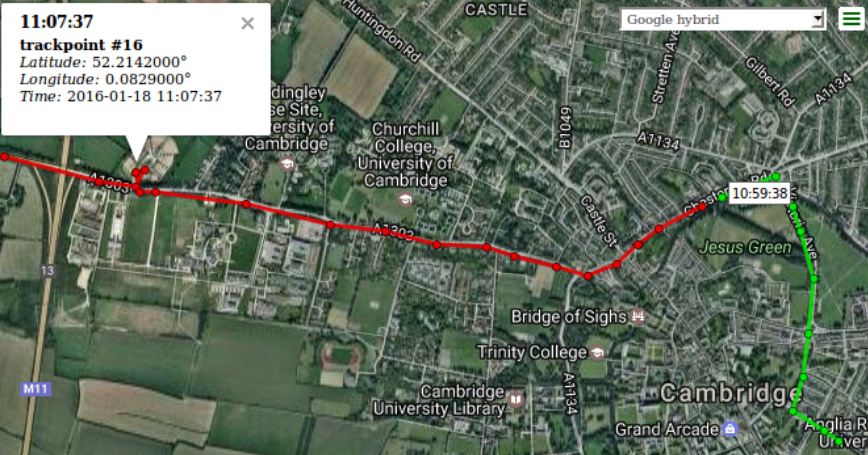
\includegraphics[width=\textwidth]{figs/madingley.png} \\

Training set having $30$ trips results in $MAE_0 = 105$s.\footnote{detailed
evaluation results are given in the appendix} \\

I now apply the optimisation nr. 1 on the same test set.\footnote{Recall that
the first optimisation predicts the arrival time from the recent trips only.
If there are no recent trips, the basic approach is used.} Looking at the
detailed results in the appendix, one can see that the
optimisation nr. 1 gives a big improvement for certain trips (e.g. the
prediction error drops from $380$s. to $40$s.) and leaves everything else
unchanged. Overall, this optimisation reduces the average prediction error to
$MAE_1 = 88$s. \\

Finally, I add the second optimisation to predict the arrival time.\footnote{The
second optimisation takes into account only equally congested historical trips.}
Both the 1st and 2nd optimisations together further reduce the average
prediction error to $MAE_{1,2} = 69$s. \\

Hence, I conclude that for this route the optimisations are worth to be applied.

\newpage

\subsection*{Comparison with the Timetable}

The prediction system is useful if for a particular route it is more accurate than
the timetable. A company named Traffi, which targets the same arrival time prediction
problem as me, agreed to share their traffic
data\footnote{I was given the November 2016 GPS data.}. \\

The Traffi data shows when the
bus has arrived at the stop \textbf{and also} when the bus was expected to arrive
according to the timetable. Hence, this data easily allows to my prediction
algorithm performance with the timetable. Assume the
arrival time prediction is what the timetable announces. Thus, one can view the
timetable as just an another prediction algorithm. Then the $MAE$ values for such an
algorithm are computed as usual. I compare the $MAE$ values of the 2 algorithms.
Thus, I have chosen one of the routes from their dataset and evaluated my algorithm
on that route. \\

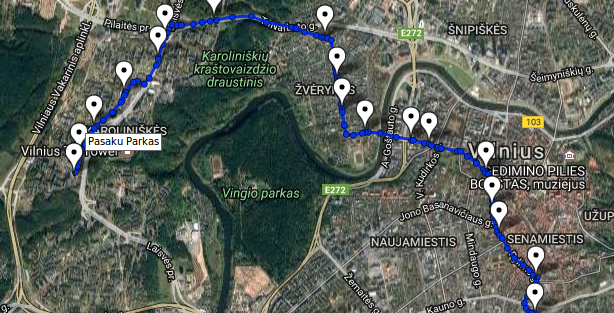
\includegraphics[width=\textwidth]{figs/vilnius_route.png} \\

The route is from my home city Vilnius. It has 18 bus stops and
I predict the arrival time to the last stop 'Pasaku Parkas' from each
of the other stops: \\


The evaluation results are shown on the next page. Two tables of errors are merged
into one and presented there. The left number of each coloured cell shows the
average prediction error of my algorithm. The right number of each coloured cell
shows the average prediction error of the timetable. \\


Note that for each column the right numbers are all the same. This is because the
arrival time announced by the timetable does not change while the bus is moving. \\

Only $4$ $MAE$ values out of $68$ are larger for my prediction algorithm. At the
beginning of the route, the bus is far away from the last stop, and I have a little amount
of recent information how it travels. That is the reason why the prediction errors
for the first stops might be worse than what the timetable announces. However,
starting from the later stops, the prediction algorithm outperforms the timetable.

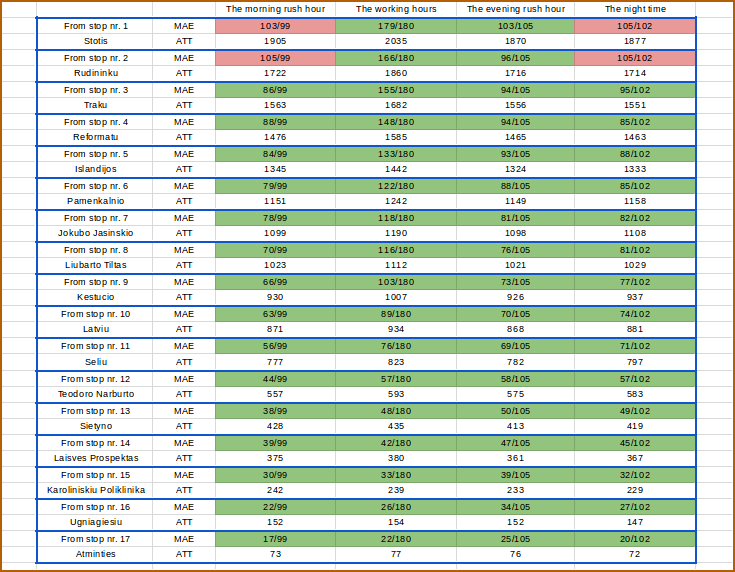
\includegraphics[width=\textwidth]{figs/table_of_vilnius.png} \\




\newpage
\section{Real-time System Evaluation (Optional)}

Suppose for a particular bus the real time system detects the route $r$ it follows.
When the bus arrives at the $b$-th bus stop, the system predicts its arrival time 
$t_{predicted}$ to the last stop of that route. The current time $t_{current}$
and the predicted time are recorded. When the bus arrives at the last stop,
the system records its actual arrival time $t_{actual}$. Thus, the system saves
as many tuples

\begin{center}
$(r, b, t_{current}, t_{predicted}, t_{actual})$
\end{center}

as possible. When I have enough tuples for a particular route $r$, I can evaluate
how well my system performs for that route. \\

I present here the evaluation of the route 1051308-20150531-22000909. The route has 10
stops. I collected $38$ buses passing through this route in 3 days. I made the arrival
time prediction to the last stop. The results are as follows: \\

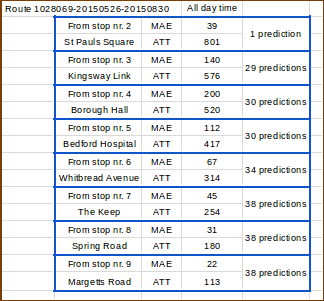
\includegraphics[scale=1.0]{figs/table_of_1051308.png}

\chapter{Conclusion}

Traffic analysis is a hot topic nowadays. In this project I had a chance to explore what it
means to deal with a large amount of GPS data. I implemented an algorithm which gives
sensible prediction results. The algorithm itself is simple, thus anyone coming after me
to improve the system should not have a trouble to read and understand what has been done
so far. \\

\section{Future Work}

Below is the list of things that I believe can improve the project most:

\begin{itemize}

\item  Get better GPS data. I worked with the data where the new point is received after
       30s. A lot of things can change in 30s. For example, a bus can arrive at the bus
       stop, briefly stop at it and depart in 30s. In that case the GPS data will not
       indicate that the bus stopped at the bus stop. Thus, I can not be sure at what exact
       time the bus actually arrived at the stop. This complicates the arrival time
       prediction evaluation. \\

       There is another problem with the current GPS data. Sometimes the GPS device gets
       "stuck". For a few minutes it reports the same bus location. After that there is
       a big change between the last and new (latitude, longitude) pairs. Finding a way
       to fix this would help.

\item  Get better route data. The routes I have are outdated. Some buses do not follow any
       of the routes present in my set.

\item  Make the real-time system process the data faster. Since I did not spend much time
       for this optional part, there is plenty of room to improve it. Currently I do not
       predict the arrival time for \textbf{each} bus in 30s. One performance bottleneck is
       the $FollowsPath$ predicate implementation. I am using it often to make sure that
       the bus both follows the path and has not deviated from it. I think it is possible
       to reduce the time complexity from $O(nm)$ to $O(n + m)$, where $n$ is the number of
       recent sub-trip points, m is the number of historical path points. This reduction
       would allow me to process significantly more buses in 30s.

       Another thing worth considering is to parallelise the system. My system is built in
       a way that for each bus I independently predict its arrival time to future stops.
       In the best case (if the lab has enough computation resources), one can consider
       dedicating a separate core per bus.

\end{itemize}

%%%%%%%%%%%%%%%%%%%%%%%%%%%%%%%%%%%%%%%%%%%%%%%%%%%%%%%%%%%%%%%%%%%%%
% the appendices
\appendix

\chapter{Links}

\begin{enumerate}
\item Dynamic time warping is an algorithm for measuring similarity between
two temporal sequences which may vary in speed. For instance, similarities in
walking could be detected using DTW, even if one person was walking faster than
another. I used DTW algorithm as a core part to implement my $FollowsPath$
predicate, with $err$ function being used instead of a regular distance function 
$d(x, y)$.
For more info look at

\textcolor{blue}{\url{https://en.wikipedia.org/wiki/Dynamic_time_warping}}

\item Project code can be found at: 

\textcolor{blue}{\url{https://github.com/ml693/bus}}


\end{enumerate}

\chapter{Detailed Evaluation Results}

\section{Multiple Routes Evaluation}

\label{B1}

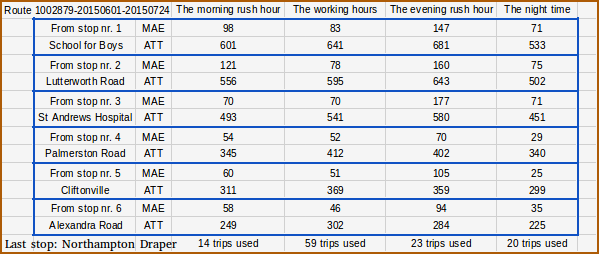
\includegraphics[width=\textwidth]{figs/table_of_1002879.png}
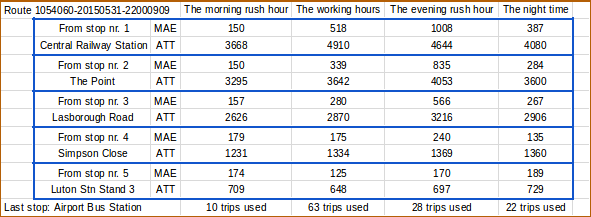
\includegraphics[width=\textwidth]{figs/table_of_1054060.png}
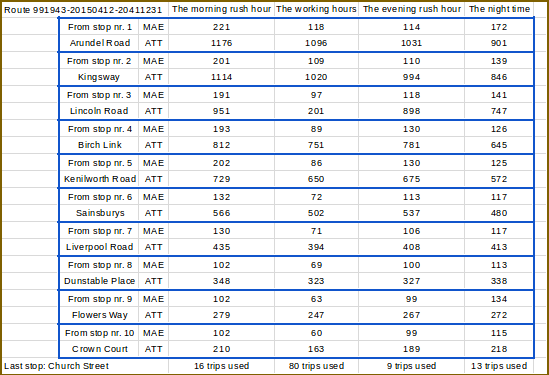
\includegraphics[width=\textwidth]{figs/table_of_991943.png}
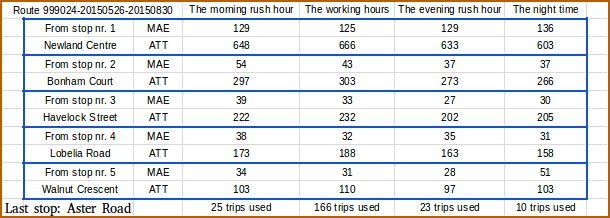
\includegraphics[width=\textwidth]{figs/table_of_999024.png}
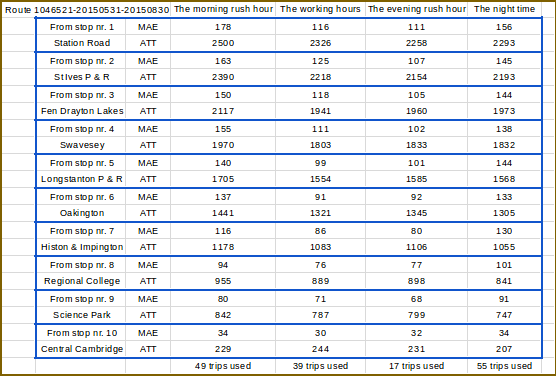
\includegraphics[width=\textwidth]{figs/table_of_1046521.png}
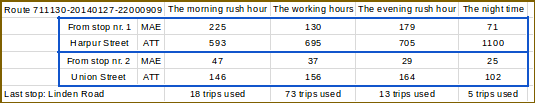
\includegraphics[width=\textwidth]{figs/table_of_711130.png}
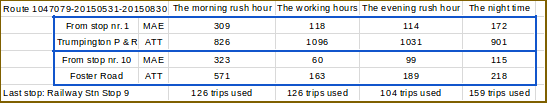
\includegraphics[width=\textwidth]{figs/table_of_1047079.png}
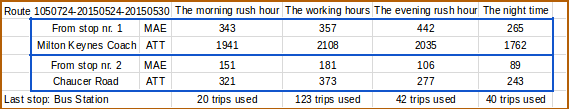
\includegraphics[width=\textwidth]{figs/table_of_1050724.png}
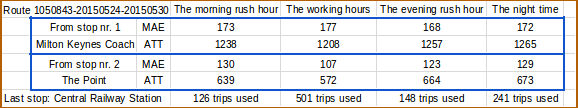
\includegraphics[width=\textwidth]{figs/table_of_1050843.png}
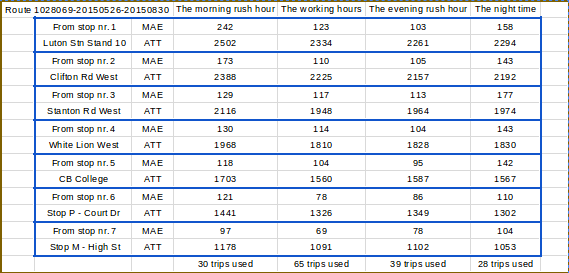
\includegraphics[width=\textwidth]{figs/table_of_1028069.png}
\includegraphics[width=\textwidth]{figs/table_of_1053969.png}
\includegraphics[width=\textwidth]{figs/table_of_1001579.png}
\includegraphics[width=\textwidth]{figs/table_of_1056213.png}
\includegraphics[width=\textwidth]{figs/table_of_1026152.png}
\includegraphics[width=\textwidth]{figs/table_of_1030740.png}
\includegraphics[width=\textwidth]{figs/table_of_1047094.png}
\includegraphics[width=\textwidth]{figs/table_of_1050847.png}
\includegraphics[width=\textwidth]{figs/table_of_1051308.png}
\includegraphics[width=\textwidth]{figs/table_of_992088.png}
\includegraphics[width=\textwidth]{figs/table_of_830638.png}
\includegraphics[width=\textwidth]{figs/table_of_1030920.png}
\includegraphics[width=\textwidth]{figs/table_of_1054599.png}
\includegraphics[width=\textwidth]{figs/table_of_1050762.png}
\includegraphics[width=\textwidth]{figs/table_of_1039292.png}
\includegraphics[width=\textwidth]{figs/table_of_1046531.png}

\newpage

\section{Predictions for Madingley Park}

Results without optimisations: \\

{\footnotesize
day18-bus14365-subtrip0 started at 2016-01-18 13:45:46, arrived at 2016-01-18 13:52:06, prediction error is -80 \\
day18-bus14368-subtrip2 started at 2016-01-18 21:14:38, arrived at 2016-01-18 21:21:18, prediction error is -60 \\
day18-bus14366-subtrip0 started at 2016-01-18 11:46:35, arrived at 2016-01-18 11:55:36, prediction error is 81 \\
day18-bus14369-subtrip1 started at 2016-01-18 17:46:33, arrived at 2016-01-18 17:55:13, prediction error is 59 \\
day18-bus403-subtrip0 started at 2016-01-18 11:23:07,    arrived at 2016-01-18 11:28:07, prediction error is -60 \\
day18-bus14374-subtrip0 started at 2016-01-18 16:15:35, arrived at 2016-01-18 16:22:35, prediction error is 19 \\
day18-bus14361-subtrip0 started at 2016-01-18 10:16:14, arrived at 2016-01-18 10:28:34, prediction error is 340 \\
day18-bus14370-subtrip0 started at 2016-01-18 10:30:47, arrived at 2016-01-18 10:44:47, prediction error is \textcolor{red}{\textbf{380}} \\ 
day18-bus14365-subtrip1 started at 2016-01-18 21:44:37, arrived at 2016-01-18 21:50:17, prediction error is -80 \\
day18-bus407-subtrip1 started at 2016-01-18 10:15:37,    arrived at 2016-01-18 10:28:40, prediction error is 334 \\
day18-bus14368-subtrip1 started at 2016-01-18 13:14:46, arrived at 2016-01-18 13:20:06, prediction error is -100 \\
day18-bus14363-subtrip1 started at 2016-01-18 15:46:05, arrived at 2016-01-18 15:53:45, prediction error is -20 \\
day18-bus14375-subtrip0 started at 2016-01-18 15:14:50, arrived at 2016-01-18 15:21:10, prediction error is -69 \\
day18-bus401-subtrip2 started at 2016-01-18 11:46:37,    arrived at 2016-01-18 11:55:38, prediction error is 81 \\
day18-bus14370-subtrip3 started at 2016-01-18 19:30:41, arrived at 2016-01-18 19:38:42, prediction error is 121 \\
day18-bus410-subtrip0 started at 2016-01-18 16:15:38,    arrived at 2016-01-18 16:22:38, prediction error is 20 \\
day18-bus402-subtrip0 started at 2016-01-18 10:30:38,    arrived at 2016-01-18 10:44:37, prediction error is \textcolor{red}{\textbf{379}} \\
day18-bus14373-subtrip0 started at 2016-01-18 16:46:02, arrived at 2016-01-18 16:53:42, prediction error is -1 \\
day18-bus14372-subtrip1 started at 2016-01-18 14:14:19, arrived at 2016-01-18 14:20:19, prediction error is -120 \\
day18-bus14367-subtrip2 started at 2016-01-19 00:35:49, arrived at 2016-01-19 00:40:49, prediction error is -160 \\
day18-bus14378-subtrip0 started at 2016-01-18 11:00:21, arrived at 2016-01-18 11:07:41, prediction error is 20 \\
day18-bus402-subtrip1 started at 2016-01-18 19:30:08,    arrived at 2016-01-18 19:38:37, prediction error is 89 \\
day18-bus400-subtrip0 started at 2016-01-18 10:59:38,    arrived at 2016-01-18 11:07:37, prediction error is 29 \\
day18-bus14087-subtrip0 started at 2016-01-18 09:30:34, arrived at 2016-01-18 09:36:34, prediction error is -120 \\
day18-bus409-subtrip0 started at 2016-01-18 08:25:38,    arrived at 2016-01-18 08:32:09, prediction error is -29 \\
day18-bus14371-subtrip1 started at 2016-01-18 08:54:47, arrived at 2016-01-18 09:01:07, prediction error is -70 \\
day18-bus14072-subtrip3 started at 2016-01-18 20:51:07, arrived at 2016-01-18 20:57:47, prediction error is -79 \\
day18-bus14072-subtrip1 started at 2016-01-18 12:45:18, arrived at 2016-01-18 12:53:18, prediction error is 20 \\
day18-bus14362-subtrip1 started at 2016-01-18 14:45:16, arrived at 2016-01-18 14:50:36, prediction error is -81 \\
day18-bus405-subtrip2 started at 2016-01-18 13:46:07,    arrived at 2016-01-18 13:52:08, prediction error is -59 \\
}

\newpage

Results with the optimisation nr. $1$: \\
{\footnotesize
day18-bus14365-subtrip0 started at 2016-01-18 13:45:46, arrived at 2016-01-18 13:52:06, prediction error is -80 \\
day18-bus14368-subtrip2 started at 2016-01-18 21:14:38, arrived at 2016-01-18 21:21:18, prediction error is 0 \\
day18-bus14366-subtrip0 started at 2016-01-18 11:46:35, arrived at 2016-01-18 11:55:36, prediction error is 81 \\
day18-bus14369-subtrip1 started at 2016-01-18 17:46:33, arrived at 2016-01-18 17:55:13, prediction error is 59 \\
day18-bus403-subtrip0 started at 2016-01-18 11:23:07,    arrived at 2016-01-18 11:28:07, prediction error is -60 \\
day18-bus14374-subtrip0 started at 2016-01-18 16:15:35,arrived at 2016-01-18 16:22:35, prediction error is 19 \\
day18-bus14361-subtrip0 started at 2016-01-18 10:16:14, arrived at 2016-01-18 10:28:34, prediction error is 340 \\
day18-bus14370-subtrip0 started at 2016-01-18 10:30:47, arrived at 2016-01-18 10:44:47, prediction error is \textcolor{green}{\textbf{40}} \\
day18-bus14365-subtrip1 started at 2016-01-18 21:44:37, arrived at 2016-01-18 21:50:17, prediction error is -60 \\
day18-bus407-subtrip1 started at 2016-01-18 10:15:37,    arrived at 2016-01-18 10:28:40, prediction error is 334 \\
day18-bus14368-subtrip1 started at 2016-01-18 13:14:46, arrived at 2016-01-18 13:20:06, prediction error is -100 \\
day18-bus14363-subtrip1 started at 2016-01-18 15:46:05, arrived at 2016-01-18 15:53:45, prediction error is -20 \\
day18-bus14375-subtrip0 started at 2016-01-18 15:14:50, arrived at 2016-01-18 15:21:10, prediction error is -69 \\
day18-bus401-subtrip2 started at 2016-01-18 11:46:37,    arrived at 2016-01-18 11:55:38, prediction error is 81 \\
day18-bus14370-subtrip3 started at 2016-01-18 19:30:41, arrived at 2016-01-18 19:38:42, prediction error is 121 \\
day18-bus410-subtrip0 started at 2016-01-18 16:15:38,    arrived at 2016-01-18 16:22:38, prediction error is 20 \\
day18-bus402-subtrip0 started at 2016-01-18 10:30:38,    arrived at 2016-01-18 10:44:37, prediction error is \textcolor{green}{\textbf{39}} \\
day18-bus14373-subtrip0 started at 2016-01-18 16:46:02, arrived at 2016-01-18 16:53:42, prediction error is -1 \\
day18-bus14372-subtrip1 started at 2016-01-18 14:14:19, arrived at 2016-01-18 14:20:19, prediction error is -31 \\
day18-bus14367-subtrip2 started at 2016-01-19 00:35:49, arrived at 2016-01-19 00:40:49, prediction error is -160 \\
day18-bus14378-subtrip0 started at 2016-01-18 11:00:21, arrived at 2016-01-18 11:07:41, prediction error is -200 \\
day18-bus402-subtrip1 started at 2016-01-18 19:30:08,    arrived at 2016-01-18 19:38:37, prediction error is 89 \\
day18-bus400-subtrip0 started at 2016-01-18 10:59:38,    arrived at 2016-01-18 11:07:37, prediction error is -241 \\
day18-bus14087-subtrip0 started at 2016-01-18 09:30:34, arrived at 2016-01-18 09:36:34, prediction error is -120 \\
day18-bus409-subtrip0 started at 2016-01-18 08:25:38,    arrived at 2016-01-18 08:32:09, prediction error is -29 \\
day18-bus14371-subtrip1 started at 2016-01-18 08:54:47, arrived at 2016-01-18 09:01:07, prediction error is -42 \\
day18-bus14072-subtrip3 started at 2016-01-18 20:51:07, arrived at 2016-01-18 20:57:47, prediction error is -79 \\
day18-bus14072-subtrip1 started at 2016-01-18 12:45:18, arrived at 2016-01-18 12:53:18, prediction error is 20 \\
day18-bus14362-subtrip1 started at 2016-01-18 14:45:16, arrived at 2016-01-18 14:50:36, prediction error is -81 \\
day18-bus405-subtrip2 started at 2016-01-18 13:46:07,    arrived at 2016-01-18 13:52:08, prediction error is 41 \\
}

Results with the optimisations nr. $1$ and nr. $2$: \\
{\footnotesize
day18-bus14365-subtrip0 started at 2016-01-18 13:45:46, arrived at 2016-01-18 13:52:06, prediction error is -100 \\
day18-bus14368-subtrip2 started at 2016-01-18 21:14:38, arrived at 2016-01-18 21:21:18, prediction error is -20 \\
day18-bus14366-subtrip0 started at 2016-01-18 11:46:35, arrived at 2016-01-18 11:55:36, prediction error is 41 \\
day18-bus14369-subtrip1 started at 2016-01-18 17:46:33, arrived at 2016-01-18 17:55:13, prediction error is 40 \\
day18-bus403-subtrip0 started at 2016-01-18 11:23:07,    arrived at 2016-01-18 11:28:07, prediction error is -59 \\
day18-bus14374-subtrip0 started at 2016-01-18 16:15:35, arrived at 2016-01-18 16:22:35, prediction error is 0 \\
day18-bus14361-subtrip0 started at 2016-01-18 10:16:14,arrived at 2016-01-18 10:28:34, prediction error is 280 \\
day18-bus14370-subtrip0 started at 2016-01-18 10:30:47, arrived at 2016-01-18 10:44:47, prediction error is 40 \\
day18-bus14365-subtrip1 started at 2016-01-18 21:44:37, arrived at 2016-01-18 21:50:17, prediction error is -51 \\
day18-bus407-subtrip1 started at 2016-01-18 10:15:37,    arrived at 2016-01-18 10:28:40, prediction error is 302 \\
day18-bus14368-subtrip1 started at 2016-01-18 13:14:46, arrived at 2016-01-18 13:20:06, prediction error is -100 \\
day18-bus14363-subtrip1 started at 2016-01-18 15:46:05, arrived at 2016-01-18 15:53:45, prediction error is -20 \\
day18-bus14375-subtrip0 started at 2016-01-18 15:14:50, arrived at 2016-01-18 15:21:10, prediction error is -42 \\
day18-bus401-subtrip2 started at 2016-01-18 11:46:37,    arrived at 2016-01-18 11:55:38, prediction error is 60 \\
day18-bus14370-subtrip3 started at 2016-01-18 19:30:41, arrived at 2016-01-18 19:38:42, prediction error is 122 \\
day18-bus410-subtrip0 started at 2016-01-18 16:15:38,    arrived at 2016-01-18 16:22:38, prediction error is 20 \\
day18-bus402-subtrip0 started at 2016-01-18 10:30:38,    arrived at 2016-01-18 10:44:37, prediction error is 39 \\
day18-bus14373-subtrip0 started at 2016-01-18 16:46:02, arrived at 2016-01-18 16:53:42, prediction error is -20 \\
day18-bus14372-subtrip1 started at 2016-01-18 14:14:19, arrived at 2016-01-18 14:20:19, prediction error is -31 \\
day18-bus14367-subtrip2 started at 2016-01-19 00:35:49, arrived at 2016-01-19 00:40:49, prediction error is -180 \\
day18-bus14378-subtrip0 started at 2016-01-18 11:00:21, arrived at 2016-01-18 11:07:41, prediction error is 20 \\
day18-bus402-subtrip1 started at 2016-01-18 19:30:08,    arrived at 2016-01-18 19:38:37, prediction error is 108 \\
day18-bus400-subtrip0 started at 2016-01-18 10:59:38,    arrived at 2016-01-18 11:07:37, prediction error is 29 \\
day18-bus14087-subtrip0 started at 2016-01-18 09:30:34, arrived at 2016-01-18 09:36:34, prediction error is -60 \\
day18-bus409-subtrip0 started at 2016-01-18 08:25:38,    arrived at 2016-01-18 08:32:09, prediction error is -9 \\
day18-bus14371-subtrip1 started at 2016-01-18 08:54:47, arrived at 2016-01-18 09:01:07, prediction error is -42 \\
day18-bus14072-subtrip3 started at 2016-01-18 20:51:07, arrived at 2016-01-18 20:57:47, prediction error is -81 \\
day18-bus14072-subtrip1 started at 2016-01-18 12:45:18, arrived at 2016-01-18 12:53:18, prediction error is -1 \\
day18-bus14362-subtrip1 started at 2016-01-18 14:45:16, arrived at 2016-01-18 14:50:36, prediction error is -80 \\
day18-bus405-subtrip2 started at 2016-01-18 13:46:07,    arrived at 2016-01-18 13:52:08, prediction error is -99 \\
}


\chapter{Project Proposal}
(see the next page)

\includepdf[pages=-]{proposal.pdf}

\end{document}
